\chapter{\texorpdfstring{\glsdesc{MMLT}}{MMLT}}
\label{cha:mmlt}
Subsequently, we get on to the main problem of this thesis: the
\gls{MMLT}. This \namecref{cha:mmlt} covers its complexity, mentions
different potential approaches, and finally presents an algorithm
for solving it. Let us begin with a formal definition of the problem
by reducing it to the Point Set Triangulation
(\cref{def:point_set_triangulation}):

\begin{problem}[\gls{MMLT}]
  \label{prob:mmlt}\hfill
  \begin{labeling}{\hspace{4em}}
    \item[\textbf{Given:}]
      Set of points \(P\), length function \(|s|\)
      for each line segment \(s\) with endpoints in \(P\)
      (e.g. Euclidean distance of the endpoints)
    \item[\textbf{Sought:}]
      Point Set Triangulation \(\gls{Topt} = T(P)\) of \(P\)
      which maximizes \(\min\limits_{s\in \gls{Topt}} |s|\)
  \end{labeling}
\end{problem}

A first observation being made is that an optimal solution for
\gls{MMLT} needs not be unique, i.e. there can be multiple solutions
\gls{Topt} with the same value for the shortest segment in \gls{Topt}.
See also \cref{fig:non_unique_optimal} for an example.

\begin{figure}[ht]
  \centering
  \begin{subfigure}{0.25\textwidth}
    \centering
    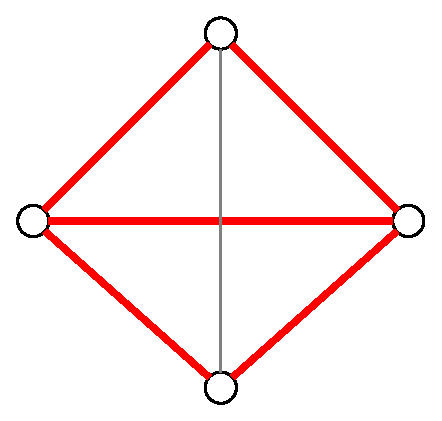
\includegraphics[width=\textwidth]{img/non_unique_optimal_1.pdf}
  \end{subfigure}
  \hspace{2em}
  \VRule
  \hspace{2em}
  \centering
  \begin{subfigure}{0.25\textwidth}
    \centering
    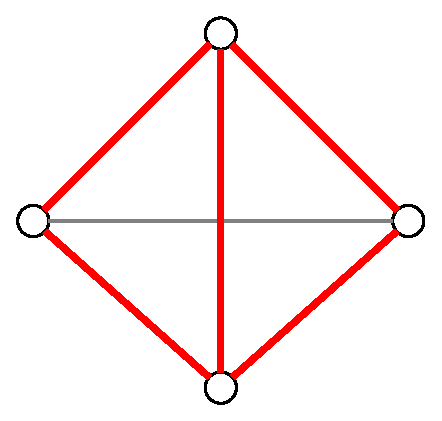
\includegraphics[width=\textwidth]{img/non_unique_optimal_2.pdf}
  \end{subfigure}
  \caption{\label{fig:non_unique_optimal}%
    Example of different optimal \gls{MMLT} solutions %
    for the same point set using Euclidean distance of the endpoints %
    as length for each line segment}
\end{figure}

\section{Complexity}
\label{sec:mmlt_complexity}
As already mentioned in \cref{sec:related_work}, the \gls{MMLT}
problem was stated as an open problem by Edelsbrunner and Tan in
1991~\cite{triangulation_minmax_length} and has recently been proven
to be NP-hard by Fekete~\cite{mmlt_complexity}. In the following, we
briefly sketch the proof.

Firstly, we adopt the definition of the \gls{CDS} problem which has
been part of~\cite{mmlt_complexity} and which we will need
afterwards:

\begin{problem}[\gls{CDS}]
  \label{prob:cds}\hfill
  \begin{labeling}{\hspace{4em}}
    \item[\textbf{Given:}]
      Set of line segments \(S\), 
      set of target points
      \(T \subseteq \{ s_i \cap s_j : s_i,s_j \in S \} \)
    \item[\textbf{Sought:}]
      Set of non-intersecting line segments
      \(\gls{Sopt} \subseteq S\) such that \(T\) is covered:
      \[ \forall p \in T: \exists s \in \gls{Sopt} : p \in s \]
  \end{labeling}
\end{problem}

It can be shown that \gls{CDS} is NP-complete---which we will skip at
this point:

\begin{theorem}[NP-completeness of \gls{CDS}]
  \label{thm:complexity_cds}
  \Cref{prob:cds} (\gls{CDS}) is NP-complete.
  \begin{proof}
  \gls{CDS} can be reduced to Planar 3-SAT (\cref{prob:planar_3SAT})
  and vice-versa. Therefore we construct a \gls{CDS} instance from
  the planar variable-clause-connection graph of a Planar 3-SAT
  instance. Each variable vertex gets replaced by a cycle of target
  points which are connected by line segments which alternating
  represent assigning either true or false to the variable.
  Additionally, the target points contain all clause vertices which
  are the intersection point of three long segments intersecting
  the respective assignment line segment of the variables taking
  part in the clause. See \cref{fig:example_CDS} for an example of
  such a construction. Note that this construction can be done in
  polynomial time and the \gls{CDS} can be solved if and
  only if there is an assignment to the Planar 3-SAT variables which
  lets all clauses evaluate to ``true''.
  For further details of the proof refer to~\cite{mmlt_complexity}.
  \end{proof}
\end{theorem}

\begin{figure}[ht]
  \centering
  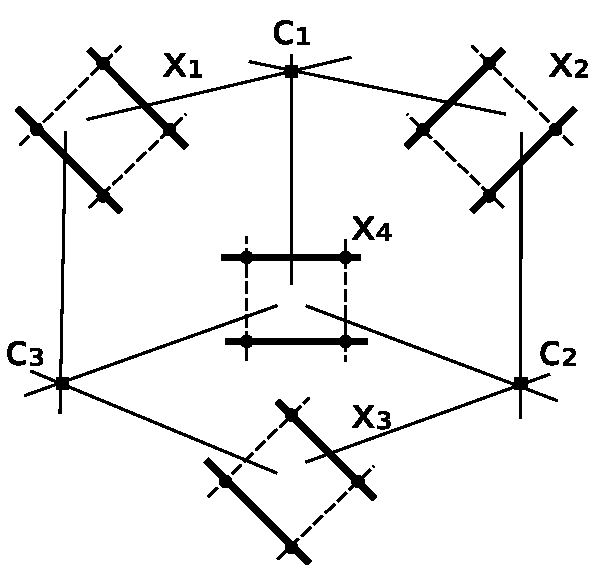
\includegraphics[width=0.5\textwidth]{img/example_CDS.pdf}
  \caption{\label{fig:example_CDS}Example of a \gls{CDS} construction 
    for the Planar 3-SAT instance from \cref{fig:example_planar_3SAT}, 
    bold line segments represent assignment of variables to ``true'',
    dashed line segments represent ``false'', and long line segments
    connected clauses with the respective variable assignments}
\end{figure}

Now we can proceed with the \gls{MMLT} problem:

\begin{theorem}[NP-hardness of \gls{MMLT}]
  \Cref{prob:mmlt} (\gls{MMLT}) is NP-hard---even for the case
  where \(P\) is planar.
  \begin{proof}
  We summarize the reduction from \gls{CDS} to \gls{MMLT}
  of~\cite{mmlt_complexity}. Let us continue from the construction of
  the proof for \cref{thm:complexity_cds}. We assume that three points
  are collinear only if they correspond to the endpoints of a line
  segment \(s\) and a target point covered by \(s\) (this can be
  achieved by perturbation). Furthermore, let \(\delta\) be the
  minimum distance of any point to a line segment it is not part of
  and assume that every line segment has at least length \(\delta\)
  (can be achieved by appropriate scaling). We now replace every
  target point of the \gls{CDS} instance by a tuple of points with
  distance \(\epsilon\) such that \(\epsilon \ll \delta\).
  
  The shortest line segment in an optimal \gls{MMLT} solution for the
  constructed instance has length \(\epsilon\) if and only if the
  initial \gls{CDS} has a solution. This is due to the fact that the
  only line segments of length \(\epsilon\) are those which replaced
  the target points and every other line segment is longer. From the
  definition of \gls{MMLT} follows, that every \(\epsilon\)-segment
  is part of the solution if and only if there is no \gls{cross}
  line segment in the solution. 
  
  For the \(\epsilon\)-segments which
  replaced the clause vertices, only the long line segments connecting
  a clause with its variables are \gls{cross}. This implies that the
  \(\epsilon\)-segment for a clause it part of an optimal \gls{MMLT} 
  solution if and only if the clause can satisfied in the 3-SAT
  problem (or the target point at that position can be covered in the
  \gls{CDS} problem).
  
  In a variable cycle, \(\epsilon\)-segments are only picked if
  neither all line segment representing an assignment to ``true'' nor
  all of those representing ``false'' can be part of the \gls{MMLT}
  solution. This is the case when two clauses of the 3-SAT problem
  require the variable to have conflicting assignments.
  
  Finally, let us point out that the above transformation of a
  \gls{CDS} instance into a \gls{MMLT} instance can be done in
  polynomial time such that we reduced \gls{CDS} to \gls{MMLT}---which
  implies \gls{MMLT} being NP-hard.
  \end{proof}
\end{theorem}

\section{Geometric Approaches}
In \cref{cha:triangulations} we mentioned two efficient methods for
finding Triangulations: sweep algorithms and edge flipping. Here we
shortly explain why these approaches can not directly be applied to
the \gls{MMLT} problem.

Sweep algorithms compute solutions for geometric problems (usually in
the plan) gradually and rely on the assumption that every part of the
solution ``behind'' the current position of the sweep line is fixed
and needs not to be changed anymore. For the \gls{MMLT} problem, the
last line segment reached by the sweep line may change for every line
segment it crosses whether it is part of the solution---which may then
force itself an update of other line segments. Therefore no part of
the solution can be fixed until all line segments are considered which
does not comply with the idea of sweep algorithms.

For the edge flipping strategy (traversing a path in the Flip Graph)
we show an example in \cref{fig:nonoptimal_flips} which requires an
edge flip to worsen the \gls{MMLT} before the optimal solution can be
reached. This essentially requires that every edge flip of the whole
Flip Graph has to be considered---which leads to exponential running
time.

\begin{figure}[ht]
  \centering
  \begin{subfigure}{0.4\textwidth}
    \centering
    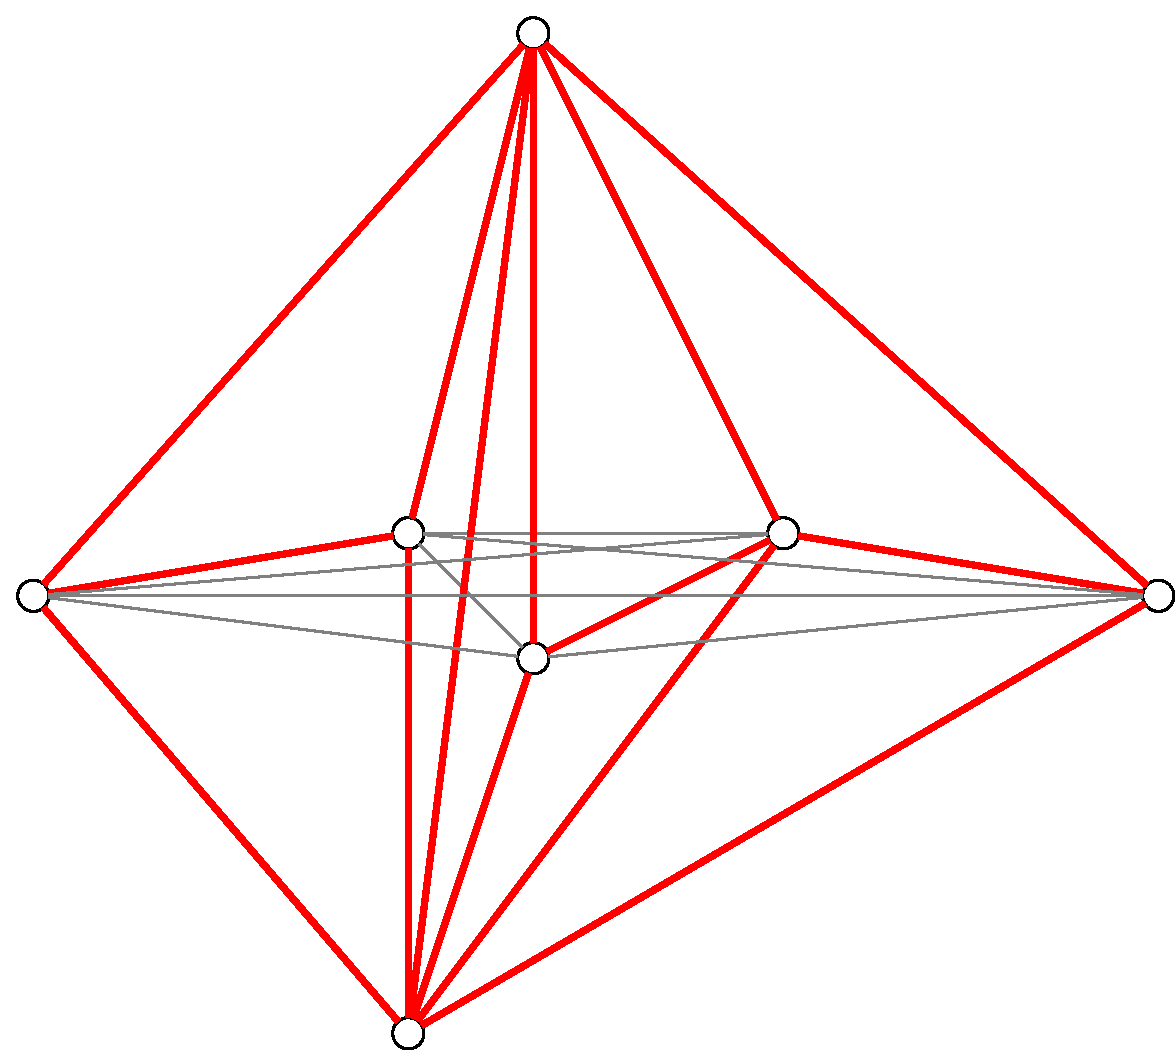
\includegraphics[width=\textwidth]{img/nonoptimal_flips_1.pdf}
  \end{subfigure}
  \hspace{1em}
  \VRule
  \hspace{1em}
  \centering
  \begin{subfigure}{0.4\textwidth}
    \centering
    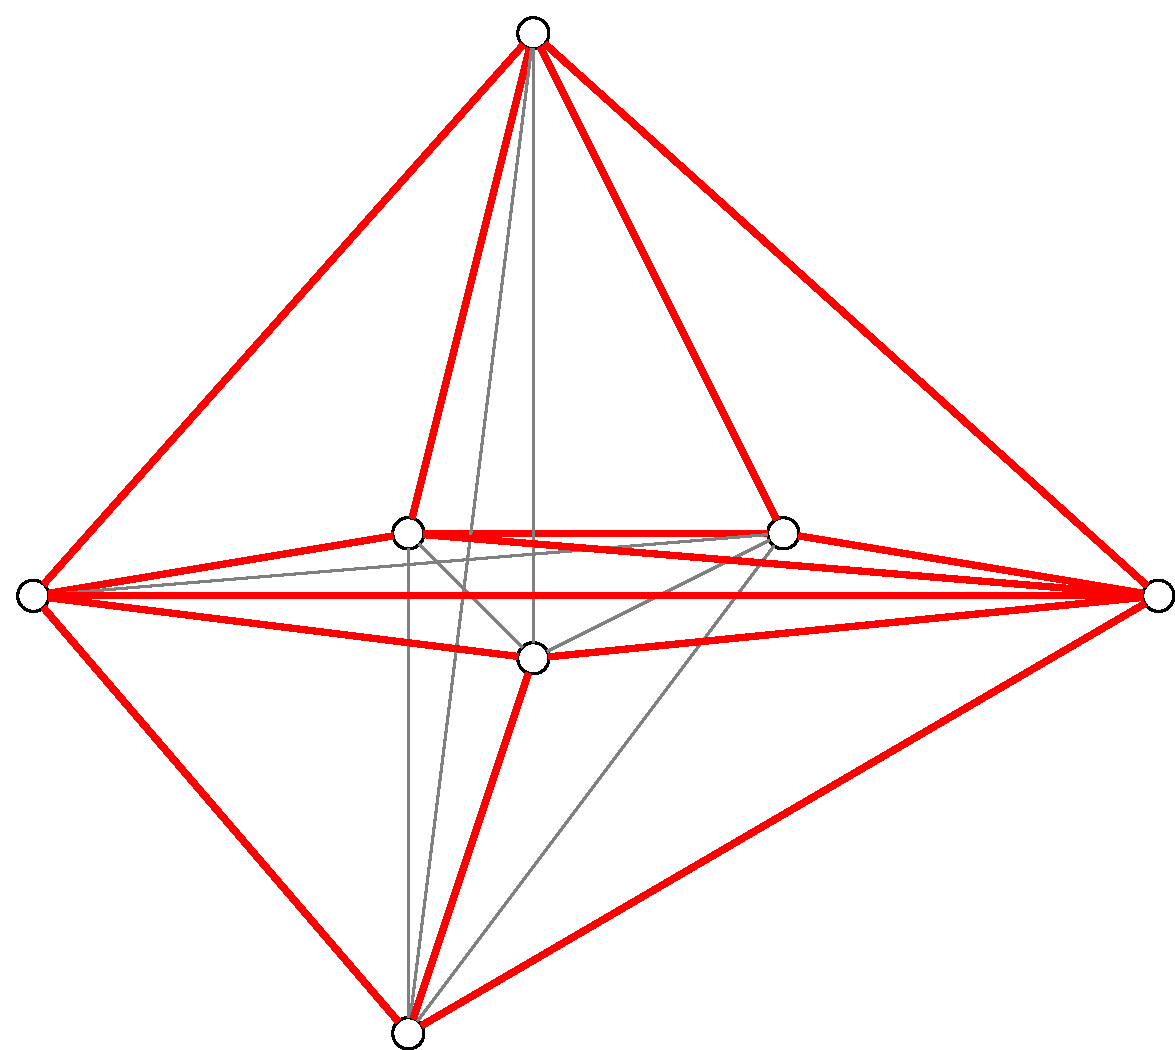
\includegraphics[width=\textwidth]{img/nonoptimal_flips_2.pdf}
  \end{subfigure}
  \caption{\label{fig:nonoptimal_flips}Example of necessary locally
    non--optimal flips: The shortest edge needs to be flipped in
    before the optimal solution can be achieved.}
\end{figure}

\section{Combinatorial Approach}
\label{sec:combinatorial_approach}
In this \namecref{sec:combinatorial_approach}, we demonstrate an
alternative way of finding optimal \gls{MMLT} solutions based on the
underlying combinatorial problem. We come up with another problem, the
\gls{MELT}, which is similar to \gls{MMLT} yet solely combinatorial.

First of all, we define a new strict total order on the potential
edges of a triangulation to circumvent the fact that two different
line segments can have the same length which implies that two optimal
\gls{MMLT} solutions may have a different shortest line segment.

\begin{definition}[Edge Length Order]
  \label{def:edge_length_order}
  Given a set of edges \(E\) representing a set of line segments
  \(S\) and two edges \(e_{s_i}, e_{s_j} \in E\) representing two
  line segments \(s_i,s_j \in S\), respectively. Let \(|s|\) for
  \(s \in S\) be the segment length and \( s_i < s_j \) the
  lexicographical order of \(s_i, s_j \in S\). The \emph{Edge Length
  Order} is defined as  
  \[
    e_{s_i} < e_{s_j}
    \iff |s_i| < |s_j|
    \lor ((|s_i| = |s_j|) \land (s_i < s_j)).
  \]
\end{definition}

Furthermore, we define a short cut for the position that an edge has
in a set sorted by the Edge Length Order which can be seen as a
higher level length function.

\begin{definition}[Edge Length Index]
  \label{def:edge_length_index}
  Given a set of edges \(E\) representing a set of line segments
  \(S\) and an edge \(e \in E\). The \emph{Edge Length Index}
  \(\idx(e)\) is the index of \(e\) in \(E\) sorted by 
  Edge Length Order.
\end{definition}

As a side effect of the Edge Length Order, we can now address every
edge in a set uniquely by its Edge Length Index which we state in the
following \namecref{thm:edge_length_index_uniqueness}.

\begin{theorem}[Uniqueness of Edge Length Index]
  \label{thm:edge_length_index_uniqueness}
  For a set of edges \(E\) representing line segments \(S\),
  there can be no two different edges \(e, e' \in E\)
  with the same Edge Length Index.
  \begin{proof}
  For two two segments \(s, s' \in S\) the lexicographical order is
  unique---i.e. either \(s < s'\) or \(s > s'\) but not both. The
  same holds for the Edge Length Order.
  \end{proof}
\end{theorem}

Using the Edge Length Index for the Triangulation edges instead of
the line segment length, we can now formulated the combinatorial
equivalent of the \gls{MMLT} problem:

\begin{problem}[\gls{MELT}]
  \label{prob:melt}\hfill
  \begin{labeling}{\hspace{4em}}
    \item[\textbf{Given:}]
      Set of points \(P\)
    \item[\textbf{Sought:}]
      Point Set Triangulation \(\gls{Topt} = T(P)\) of \(P\)
      which maximizes the minimum Edge Length Index
      \(\min\limits_{e\in \gls{Topt}} \idx(e)\).
  \end{labeling}
\end{problem}

Even though, there can still be arbitrary many optimal \gls{MELT}
solutions (as for \gls{MMLT}) at least the ``shortest'' edge (meaning
the one with minimum Edge Length Index) is the same in all of them.
Because neither the \gls{MMLT} nor the \gls{MELT} problem ask for the
whole vector of edges to be maximum, there can still be different
combinations of edges with higher Edge Length Index.

\begin{theorem}[Uniqueness of Optimal \gls{MELT} Solutions]
  \label{thm:melt_uniqueness}
  From \Cref{thm:edge_length_index_uniqueness} follows directly that
  every optimal solution for \cref{prob:melt} (\gls{MELT}) has the
  same edge with minimum Edge Length Index.
\end{theorem}

Even though the link between \gls{MMLT} and \gls{MELT} may be obvious,
the proof is yet to come and covered by the following
\namecref{thm:equality_melt_mmlt}.

\begin{theorem}[Equality of \gls{MELT} and \gls{MMLT}]
  \label{thm:equality_melt_mmlt}
  Every optimal \gls{MELT} solution is an optimal \gls{MMLT} solution.
  \begin{proof}
  Let \gls{Topt} be an optimal \gls{MELT} solution
  for a point set \(P\) and assume that that
  there is a \gls{MMLT} solution \(T\) with
  \(\min\limits_{s \in T} |s| < \min\limits_{s \in \gls{Topt}} |s|\).
  By \cref{def:edge_length_index,def:edge_length_order}
  \( \idx(\argmin\limits_{s \in T} |s|)
    < \idx(\argmin\limits_{s \in \gls{Topt}} |s|) \)---which
    contradicts \gls{Topt} being optimal.
  \end{proof}
\end{theorem}

Now the complexity of \gls{MELT} is straightforward as a reduction
from \gls{MMLT} can easily be done considering
\cref{thm:equality_melt_mmlt}. Compare also \cref{sec:mmlt_complexity}
for further details of the complexity of the \gls{MMLT} problem.

\begin{theorem}[NP-hardness of \gls{MELT}]
  From \cref{thm:equality_melt_mmlt} follows
  that \gls{MELT} is NP-hard.
\end{theorem}

Despite the fact that \gls{MMLT} instances can be solved through the
corresponding \gls{MELT} problem, there is one important difference
between both problems that we will exploit in the following: Making
use of the Edge Length Index, \gls{MELT} instances contain only
integers. This allows us to transform the problem into an \gls{IP}
(see also \cref{cha:integer_programming}).

\begin{problem}[\gls{IP} Formulation of \gls{MELT}]
  \hfill
  \begin{alignat*}{1}
    E: &~ \text{\gls{noverlap} line segments with endpoints in \(P\)} \\
    X: &~ \text{pairs of \gls{cross} line segments} \\
    T: &~ \text{\gls{MELT} solution}
  \end{alignat*}
  \begin{alignat*}{3}
    &\text{maximize } & \min\limits_{e \in T} x_e \cdot \idx(e) \\
    &\text{subject to } & \forall \{e_i,e_j\} \in X : &~& x_{e_i} + x_{e_j} &\leq 1 \\
    && \forall e_i \in E : &~
      & x_{e_i} + \sum\limits_{\{e_i, e_j\} \in X} x_{e_j} &\geq 1 \\
    && \forall e \in E : &~& x_e &\in \{0,1\}
  \end{alignat*}
\end{problem}

\section{Separators}
The \gls{IP} for \gls{MELT} contains \(n^2\) variables and
\(O(n^4)\) restrictions for \(n\) points---even though most of them
are irrelevant for the optimal solution. Therefore we identify two
groups of interesting edges: \emph{Short Edges}, which are potential
candidates for the smallest Edge Length Index in an optimal
\gls{MELT} solution, and \emph{Separators}, which may avoid certain
Short Edges.

\begin{definition}[Short Edges]
  \label{def:short_edges}
  \emph{Short Edges} within a set of edges \(E\) are all edges with an
  Edge Length Index smaller than a certain threshold:
  \[
    \gls{Eshort}[(E, \ell)] := \{ e \in E : \idx(e) < \ell \}
  \]
\end{definition}
\vspace*{-1.5em}
\begin{definition}[Separators]
  \label{def:separators}
  Given a set of edges \(E\) and edge conflicts \(X \subseteq E^2\). 
  The set of \emph{Separators} \(\gls{Esep}[(E, X, e)]\) 
  for an edge \(e \in E\) are all edges
  that improve the \gls{MELT} solution, i.e. all \gls{esep} with
  \(\{e,\gls{esep}\} \in X\) which have a higher Edge Length Index:
  \[
	  \gls{Esep}[(E,X,e)] := \{
		  \gls{esep} \in E:
		  \idx(e) < \idx(\gls{esep}) \land \{e,\gls{esep}\} \in X
	  \}
  \]
\end{definition}

The preceding \cref{def:short_edges,def:separators} allow us to
restrict the edges that may influences an optimal \gls{MELT} solution
\gls{Topt} such that we can formulate an upper bound on the minimum
Edge Length Index in \gls{Topt}.

\begin{theorem}[Upper Bound for \gls{MELT}]
  \label{thm:upper_bound}
  Given the optimal \gls{MELT} solution \gls{Topt}
  for a point set \(P\), let \(E\) be all \gls{noverlap} line segments
  contained in the Complete Graph \(K_{V(P)}\)
  where \(V(P)\) represents \(P\),
  and let \(X\) all conflicts in the Intersection Graph of \(P\).
  Every edge \(e \in E\) without Separators
  is an upper bound for \gls{Topt}:
  \[
    \forall e \in E,~ \gls{Esep}[(E,X,e)] = \emptyset :
    \min\limits_{\gls{emin} \in \gls{Topt}}
    \idx(\gls{emin}) \leq \idx(e)
  \]
  which is equivalent to
  \begin{alignat*}{1}
    \forall e \in E:~ 
    &\lnot\exists \gls{esep} \in E:
    \idx(e) < \idx(\gls{esep})
    \land~ \{e, \gls{esep}\} \in X \\
    &\implies \min\limits_{\gls{emin} \in \gls{Topt}}
    \idx(\gls{emin}) \leq \idx(e)
  \end{alignat*}
  \begin{proof}
  Assume
  \[
    \exists e \in E,~ \gls{Esep}[(E,X,e)] = \emptyset :
    \min\limits_{\gls{emin} \in \gls{Topt}}
    \idx(\gls{emin}) > \idx(e)
  \]
  This implies \(e \not\in \gls{Topt}\) and
  \[
    \forall e' \in E:
    \idx(e') < \idx(e)
    \implies e' \not\in \gls{Topt}.
  \]
  With \(\gls{Esep}[(E,X,e)] = \emptyset\) it follows that
  \(
    \forall \{e, \gls{econf}\} \in X :
    \gls{econf} \not\in \gls{Topt}
  \).
  This means that for \gls{Topt} to be a Triangulation
  \(e\) has to be in \gls{Topt}---which is a contradiction.
  \end{proof}
\end{theorem}

From all the edges without Separators, the one with smallest
Edge Length Index is clearly the one which restricts an optimal
\gls{MELT} solution in \cref{thm:upper_bound} the most. Therefore we
give it a name such that we can refer to it later:

\begin{definition}[Shortest Non-separable Edge]
  Given a set of edges \(E\) and edge conflicts \(X \subseteq E^2\).
  The \emph{Shortest Non-separable Edge} \gls{enose} is the edge
  with the smallest Edge Length Index
  from all edges which has no Separators:
  \[ 
    \gls{enose} := \argmin\limits_{
      e \in E : \gls{Esep}[(E,X,e)] = \emptyset
    } \idx(e)
  \]
\end{definition}

\Cref{fig:upper_bound_tightness} shows an example where the upper
bound for an optimal \gls{MELT} solution in \cref{thm:upper_bound} is
not tight for \gls{enose}. However, we assume that considering
\gls{enose} is still of great help for reducing the problem size
significantly---though we have only experimental evidence by now.

\begin{theorem}[Index of \gls{enose}]
  \label{thm:index_enose}
  The Edge Length Index of the Shortest Non-separable Edge \gls{enose}
  for a random point set \(P\) of size \(n=|P|\) is at most
  \(\idx(\gls{enose}) \in O(n)\) on average.
  \begin{proof}
  The proof is still unknown to us, yet we have experimental evidence
  for this to be true (see \cref{sec:results_segments}).
  \end{proof}
\end{theorem}

\begin{figure}[ht]
  \centering
  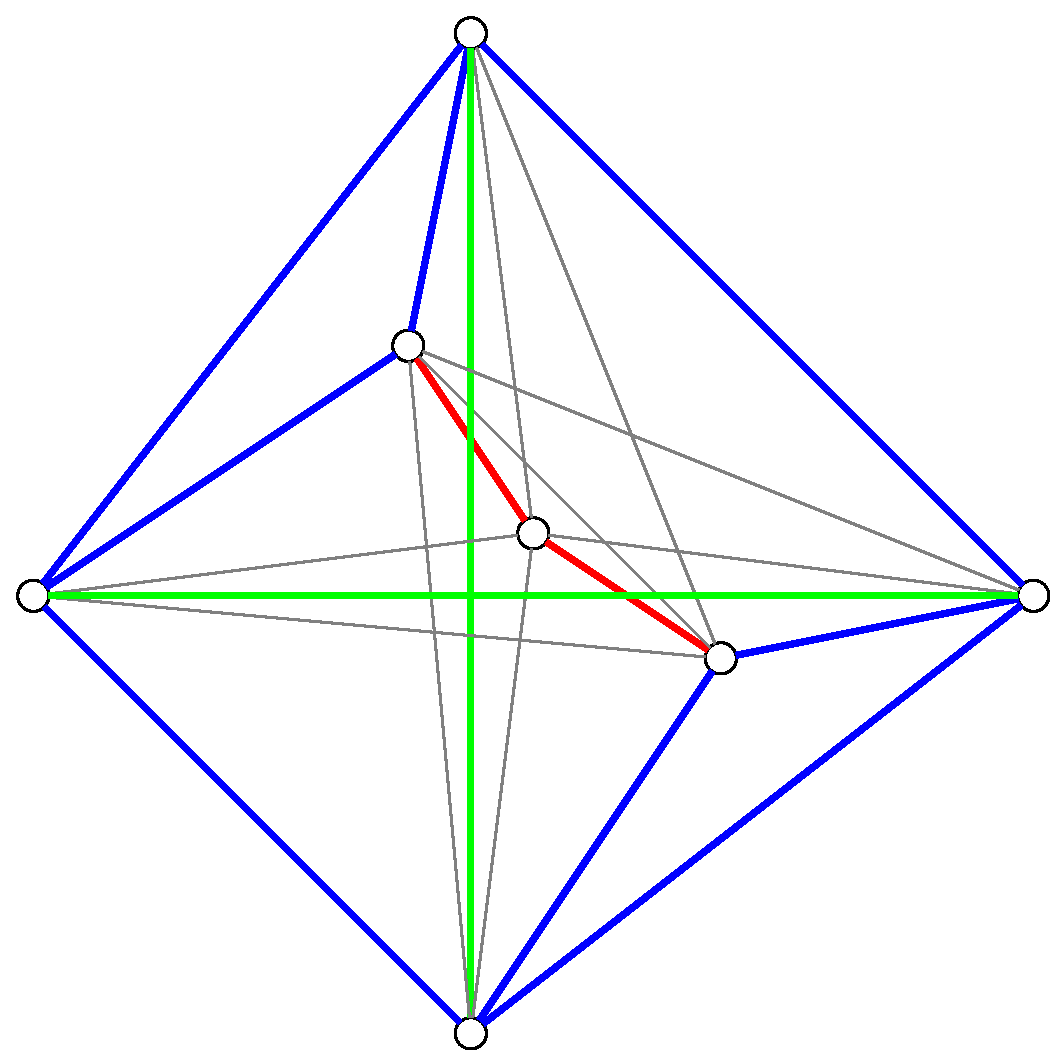
\includegraphics[width=0.5\textwidth]{img/upper_bound_tightness.pdf}
  \caption{
    \label{fig:upper_bound_tightness}
    Example where the upper bound from \cref{thm:upper_bound} is not 
    tight. One of the Short Segments (red) is part of an optimal 
    \gls{MELT} solution because their Separators (green) cross. Thus
    the shortest segment in the solution is shorter than the shortest
    one of all segments without Separators (blue).
  }
\end{figure}  

The logical consequence of \cref{thm:index_enose} is that we only need
to consider part of the edges. Our new task is to find Separators for
Short Edges where possible, which is reflected in the \gls{NOCS}
problem.

\begin{problem}[\gls{NOCS}]
  \hfill
  \begin{labeling}{\hspace{4em}}
    \item[\textbf{Given:}]
      Set of Short Edges \(E\) and their Separators \gls{Esep},
      edge conflicts \(X \subseteq (E \cup \gls{Esep})^2\)
    \item[\textbf{Sought:}]
      Set of non-conflicting edges
      \[
        \gls{Eopt} \subseteq E
        \cup \bigcup\limits_{e \in E} \gls{Esep}[(e)]
      \]
      which contains for every edge \(e \in E\) either \(e\) itself
      or at least one Separator \(\gls{esep} \in \gls{Esep}[(e)]\)
      and maximizes the smallest Edge Length Index
      \(\min\limits_{e \in \gls{Eopt}} \idx(e)\)
  \end{labeling}
\end{problem}

An essential observation at this point is that \gls{MELT} and
\gls{NOCS} pursue the same objective an lead to the same result---only
that the \gls{NOCS} solution does not contain edges which do not
influence the minimum Edge Length Index. Therefore those
``irrelevant'' edges have to be added to any optimal \gls{NOCS}
solution to retrieve an optimal \gls{MELT} solution.

\begin{theorem}[Equality of \gls{MELT} and \gls{NOCS}]
  \label{thm:equality_melt_nocs}
  Given a point set \(P\) along with all \gls{noverlap} edges \(E\)
  of the Complete Graph \(K_{V(P)}\), and all conflicts \(X\) from the
  Intersection Graph for \(E\). 
  Let \gls{enose} be the shortest non-separable edge in \(E\).
  An optimal \gls{MELT} solution \gls{Topt} for \(P\)
  and an optimal \gls{NOCS} solution \gls{Sopt} for
  \(\gls{Eshort}[(E,\idx(\gls{enose}))]\) have the same value:
  \[
    \min\limits_{e \in \gls{Topt}} \idx(e)
    = \min\limits_{e \in \gls{Sopt}} \idx(e)
  \]
  \begin{proof}
  \ldots\todo[inline]{proof?}
  \end{proof}
\end{theorem}

A direct consequence of the Shortest Non-separable Edge \gls{enose}
not being restricted in general (so it can  be the edge with highest
Edge Length Index in the worst case) is that both problems \gls{MELT}
and \gls{NOCS} have the same complexity:

\begin{theorem}[NP-hardness of \gls{NOCS}]
  For \(\gls{Eshort}[(E,\idx(\gls{enose}))] \cup \gls{enose} = E\),
  \gls{NOCS} and \gls{MELT} are the same problem.
  Therefore \gls{NOCS} is also NP-hard.
\end{theorem}

Additionally, the \gls{IP} formulation for \gls{NOCS} is also the same
as for \gls{MELT}---besides the fact that we may have less variables
and restrictions depending on the
Shortest Non-separable Edge \gls{enose}.

\begin{problem}[\gls{IP} Formulation of \gls{NOCS}]
  \hfill
  \begin{alignat*}{1}
    E: &~ \text{Short Edges} \\
    \gls{Esep}: &~ \text{Separators} \\
    X: &~ \text{edge conflicts} \\
    S: &~ \text{\gls{NOCS} solution}
  \end{alignat*}
  \begin{alignat*}{3}
    &\text{maximize } & \min\limits_{e \in S} x_e \cdot \idx(e) \\
    &\text{subject to } & \forall \{e_i,e_j\} \in X : &~& x_{e_i} + x_{e_j} &\leq 1 \\
    && \forall e_i \in E : &~
      & x_{e_i} + \sum\limits_{e_j \in \gls{Esep}[(e_i)]} x_{e_j} &\geq 1 \\
    && \forall e \in E
      \cup \bigcup\limits_{e \in E} \gls{Esep}[(e)] :
      &~& x_e &\in \{0,1\}
  \end{alignat*}
\end{problem}

Assuming that \cref{thm:index_enose} is correct, the \gls{IP} for
\gls{NOCS} is significantly smaller than for \gls{MELT} as it only has
\(O(n)\) variables and \(O(n^3)\) restrictions in case all the 
Short Edges conflict with every other edge---and
we can assume that this does not happen for random point sets.

The presence of Separators which are not necessary (i.e. which only
conflict with Short Edges already conflicting with other
Separators) in a \gls{NOCS} solution is not defined. This is what
we intend to change by introducing
\emph{complete} \gls{NOCS} solutions:

\begin{definition}[Completion of \gls{NOCS}]
  Given an optimal \gls{NOCS} solution \gls{Topt}
  for a set of Short Edges \(E\), their Separators \gls{Esep},
  and conflicts \(X\), the \emph{Completion} of \gls{Topt} is
  \[
    T := \gls{Topt} \cup \left\{
      \gls{esep} \in \bigcup\limits_{e \in E} \gls{Esep}[(e)]:
      \lnot\exists e \in T : \{e, \gls{esep}\} \in X
    \right\}.
  \]
  If \(T = \gls{Topt}\), \gls{Topt} is \emph{complete}.
\end{definition}

It is important to realize that Completion of an optimal \gls{NOCS}
solution does not destroy its optimality:

\begin{theorem}[Optimality of \gls{NOCS} Completion]
  Given an optimal \gls{NOCS} solution \gls{Topt}
  the Completion \(T\) of \gls{Topt}
  is also an optimal \gls{NOCS} solution.
  \begin{proof}
    \ldots\todo[inline]{proof?}
  \end{proof}
\end{theorem}

After we defined that ``unnecessary'' Separators may as well be in
an optimal \gls{NOCS} solution if it is complete, we can exploit the
newly acquired structure to recycle the Independent Set problem from
\cref{cha:integer_programming}:

\begin{theorem}[Connection of \gls{NOCS} and Independent Set]
  Every complete optimal \gls{NOCS} solution \gls{Topt}
  for a set of Short Edges \(E\), their Separators \gls{Esep},
  and conflicts \(X \subseteq (E \cup \gls{Esep})^2\)
  is a Maximal Independent Set (\cref{def:max_independent_set})
  for the simple graph \(G = (E \cup \gls{Esep}, X)\).
  \begin{proof}
    \ldots\todo[inline]{proof?}
  \end{proof}
\end{theorem}

\section{Algorithms}
At last, we combine earlier concepts and observations to algorithms
for solving \gls{MMLT} instances. \Cref{cha:implementation} describes
our implementation and \cref{cha:results} shows the results of running
it on random point sets. Note that (according to the common assumption
that P\(\not=\)NP) polynomial time algorithms for NP-hard
problems---and therefore also for \gls{MMLT}---are unlikely to exist.

Transforming \gls{MMLT} instances into \gls{MELT} instances requires
only for sorting the line segments by length and then by
lexicographical order to determine the Edge Length Index for every
edge. An algorithm for doing so is trivial and therefore we omit it
here.

By making use of \cref{thm:equality_melt_nocs}, we can give a
straightforward algorithm for solving \gls{MELT} instances though
reduction to \gls{NOCS}.

\begin{algorithm}
  \DontPrintSemicolon
  \KwIn{Point Set \(P\)}
  \KwOut{Optimal \gls{MELT} Solution \gls{Topt} for \(P\)}
  
  Let \(S\) be all \gls{noverlap} line segments with endpoints in \(P\) \;
  Let \(E\) be edges representing all line segments in \(S\) sorted
    by Edge Length Order \;
  Find the Shortest Non-Separable Edge \(\gls{enose} \in E\)
    and compute the partial Intersection Graph \(\gls{Gcross}[(S')] = (E',X)\)
    for all line segments \(S' \subseteq S\)
    represented by edges \(E'\)
    with \(E' = \gls{Eshort}[(E,\idx(\gls{enose}))]\) \;
  Find an optimal \gls{NOCS} solution \gls{Eopt}
    for the Short Edges \(E'\)
    with Separators \(\gls{Esep}[(E,X,e)]\) for every \(e \in E'\)
    and conflicts \(X\) \;
  Compute a Constrained Point Set Triangulation \gls{Topt}
    for \(P\) with the constraints \gls{Eopt} \;
  
  \KwRet{\gls{Topt}}
  \caption{\label{alg:melt}\gls{MELT} Algorithm}
\end{algorithm}

Constructing the partial Intersection Graph and finding the Shortest
Non-separable Edge at the same time can be done using a slightly
modified version of \cref{alg:naive_intersection} keeping the running
time of \(O(n^4)\) for \(n\) points.

Solving the \gls{NOCS} instance can be done by directly using the
\gls{IP} formulation. In our implementation however, we run a binary
search on the Edge Length Index starting with the interval 0 to
\(\idx(\gls{enose})\), and solve the corresponding decision problem
for \gls{NOCS}. This gives us the chance to abort the algorithm at any
time gaining upper and lower bound for the optimal \gls{NOCS} solution%
---and, if wanted, a ``good'' \gls{MELT} solution instead of an
optimal one.

%---------------------------------------------------------------------##########
